\chapter{Lista}

\index{lista}

\emph{Lista} (\emph{list}) on taulukkoa muistuttava muuttuvan kokoinen tietorakenne,
joka muodostuu peräkkäin olevista alkioista.
Esimerkiksi $[3,7,2,5]$ on lista, joka sisältää neljä alkiota.
Haluamme toteuttaa listan niin,
että pääsemme käsiksi listalla olevaan alkioon
sen kohdan perusteella
ja lisäksi pystymme lisäämään ja poistamaan alkioita.

Tässä luvussa tutustumme kahteen lähestymistapaan listan toteuttamiseen.
Ensin toteutamme taulukkolistan,
jossa listan alkiot tallennetaan taulukkoon.
Tämän jälkeen toteutamme linkitetyn listan,
joka muodostuu toisiinsa viittaavista solmuista.
Kuten tulemme huomaamaan, molemmissa listan toteutuksissa on omat
hyvät ja huonot puolensa.

\section{Taulukkolista}

\index{taulukkolista}

\emph{Taulukkolista} (\emph{array list}) on lista, joka on tallennettu taulukkona.
Koska taulukon alkiot ovat peräkkäin muistissa,
pääsemme käsiksi mihin tahansa listan alkioon ajassa $O(1)$.
Haasteena toteutuksessa on kuitenkin,
että taulukon koko on \emph{kiinteä} ja
listan koon muuttamiseksi täytyy varata uusi taulukko
ja kopioida sinne vanhan taulukon sisältö.

\subsection{Muutokset lopussa}

Toteutamme ensin taulukkolistan, jossa alkioiden
lisäykset ja poistot tapahtuvat listan lopussa.
Tallennamme listan taulukkona niin,
että tietty määrä alkioita taulukon alussa on listan käytössä
ja loput tyhjät kohdat on varattu tuleville alkioille.
Tämän ansiosta pystymme lisäämään uuden alkion listalle
ajassa $O(1)$, jos taulukossa on tilaa,
koska riittää ottaa käyttöön seuraava
vapaana oleva kohta taulukosta.

Kuva \ref{fig:listau} näyttää esimerkin,
jossa taulukossa on tilaa yhteensä kahdeksalle alkiolle
ja siihen on tallennettu lista $[3,7,2,5]$.
Taulukon neljä ensimmäistä kohtaa ovat siis listan käytössä
ja muut ovat varalla tulevia alkioita varten.
Kun lisäämme listan loppuun uuden alkion 6,
otamme käyttöön taulukosta uuden kohdan, johon alkio sijoitetaan.

\begin{figure}
\center
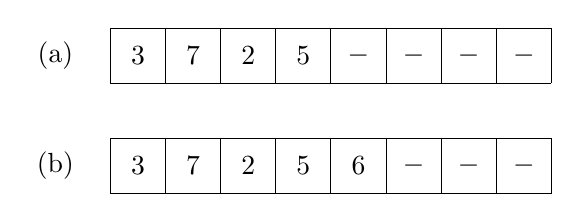
\begin{tikzpicture}[scale=0.7]
\begin{scope}
\draw (0,0) grid (8,1);
\node at (-1,0.5) {(a)};
\node at (0.5,0.5) {$3$};
\node at (1.5,0.5) {$7$};
\node at (2.5,0.5) {$2$};
\node at (3.5,0.5) {$5$};
\node at (4.5,0.5) {$-$};
\node at (5.5,0.5) {$-$};
\node at (6.5,0.5) {$-$};
\node at (7.5,0.5) {$-$};
\end{scope}
\begin{scope}[yshift=-2cm]
\draw (0,0) grid (8,1);
\node at (-1,0.5) {(b)};
\node at (0.5,0.5) {$3$};
\node at (1.5,0.5) {$7$};
\node at (2.5,0.5) {$2$};
\node at (3.5,0.5) {$5$};
\node at (4.5,0.5) {$6$};
\node at (5.5,0.5) {$-$};
\node at (6.5,0.5) {$-$};
\node at (7.5,0.5) {$-$};
\end{scope}
\end{tikzpicture}
\caption{(a) Lista $[3,7,2,5]$ tallennettuna taulukkoon. (b) Listan loppuun lisätään alkio 6.}
\label{fig:listau}
\end{figure}

\begin{figure}
\center
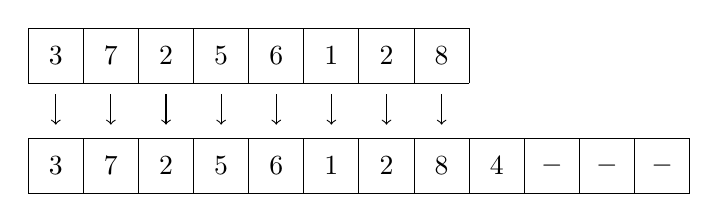
\begin{tikzpicture}[scale=0.7]
\begin{scope}
\draw (0,0) grid (8,1);
\node at (0.5,0.5) {$3$};
\node at (1.5,0.5) {$7$};
\node at (2.5,0.5) {$2$};
\node at (3.5,0.5) {$5$};
\node at (4.5,0.5) {$6$};
\node at (5.5,0.5) {$1$};
\node at (6.5,0.5) {$2$};
\node at (7.5,0.5) {$8$};
\foreach \x in {0,...,7} \draw[->] (\x+0.5,-0.2) -- (\x+0.5,-0.75);
\end{scope}
\begin{scope}[yshift=-2cm]
\draw (0,0) grid (12,1);
\node at (0.5,0.5) {$3$};
\node at (1.5,0.5) {$7$};
\node at (2.5,0.5) {$2$};
\node at (3.5,0.5) {$5$};
\node at (4.5,0.5) {$6$};
\node at (5.5,0.5) {$1$};
\node at (6.5,0.5) {$2$};
\node at (7.5,0.5) {$8$};
\node at (8.5,0.5) {$4$};
\node at (9.5,0.5) {$-$};
\node at (10.5,0.5) {$-$};
\node at (11.5,0.5) {$-$};
\end{scope}
\end{tikzpicture}
\caption{Taulukkoon ei mahdu enää uutta alkiota. Meidän täytyy varata uusi suurempi taulukko
ja kopioida vanhan taulukon sisältö sinne.}
\label{fig:lisuus}
\end{figure}

Mitä tapahtuu sitten, kun jossain vaiheessa koko taulukko
on täynnä eikä uusi listalle lisättävä alkio mahdu enää taulukkoon?
Tällöin täytyy ensin varata uusi suurempi taulukko ja
kopioida kaikki vanhan taulukon alkiot siihen,
minkä jälkeen uusi alkio voidaan lisätä listalle.
Tämä vie aikaa $O(n)$, koska kaikki listan alkiot täytyy kopioida
uuteen paikkaan muistissa.
Esimerkiksi kuvassa \ref{fig:lisuus} uusi alkio 4 ei mahdu taulukkoon,
joten joudumme varaamaan uuden taulukon ja kopioimaan alkiot.

Olemme saaneet siis aikaan listan, jossa lisääminen
vie aikaa \emph{joko} $O(1)$ tai $O(n)$ riippuen siitä,
mahtuuko alkio nykyiseen taulukkoon vai täytyykö
varata uusi taulukko.
Jotta lista olisi käyttökelpoinen, hidas $O(n)$-operaatio
ei saisi esiintyä liian usein.
Osoittautuu, että tämä tavoite toteutuu,
kunhan varaamme uuden taulukon aina reilusti aiempaa suuremmaksi.
Tyypillinen ratkaisu on \emph{kaksinkertaistaa} taulukon koko aina,
kun varaamme uuden taulukon.
Kun toimimme näin, jokaisen alkion lisääminen listalle vie
\emph{keskimäärin} vain $O(1)$ aikaa.

Miksi aikaa kuluu keskimäärin vain $O(1)$?
Tarkastellaan tilannetta, jossa listassa on $n$ alkiota
ja taulukko on tullut täyteen,
joten alkiot täytyy kopioida uuteen taulukkoon.
Tiedämme, että alkioita kopioitiin viimeksi silloin,
kun listassa oli $n/2$ alkiota,
joten listaan on lisätty välissä $n/2$ alkiota tehokkaasti.
Niinpä $n$ alkion kopioimisen kustannus voidaan jakaa
$n/2$ aiemmin lisätylle alkiolle, ja jokaiseen alkioon
kohdistuva lisäkustannus on vakio.
Taulukon kasvattamisen vaikutus kokonaisuuteen on siis pieni.

\begin{figure}
\center
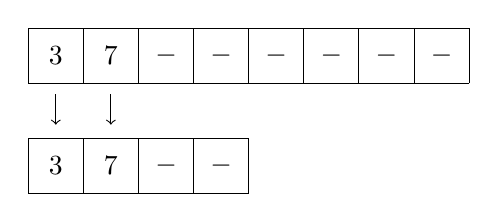
\begin{tikzpicture}[scale=0.7]
\begin{scope}
\draw (0,0) grid (8,1);
\node at (0.5,0.5) {$3$};
\node at (1.5,0.5) {$7$};
\node at (2.5,0.5) {$-$};
\node at (3.5,0.5) {$-$};
\node at (4.5,0.5) {$-$};
\node at (5.5,0.5) {$-$};
\node at (6.5,0.5) {$-$};
\node at (7.5,0.5) {$-$};
\foreach \x in {0,...,1} \draw[->] (\x+0.5,-0.2) -- (\x+0.5,-0.75);
\end{scope}
\begin{scope}[yshift=-2cm]
\draw (0,0) grid (4,1);
\node at (0.5,0.5) {$3$};
\node at (1.5,0.5) {$7$};
\node at (2.5,0.5) {$-$};
\node at (3.5,0.5) {$-$};
\end{scope}
\end{tikzpicture}
\caption{Poistojen jälkeen taulukon koko on käynyt tarpeettoman suureksi,
ja puolitamme taulukon koon.}                                                                        
\label{fig:lispoi}
\end{figure}

Voimme poistaa alkion listan lopusta aina $O(1)$-ajassa,
koska taulukon kokoa ei tarvitse koskaan suurentaa.
Tässä voi kuitenkin tulla ongelmaksi, että monien poistojen
jälkeen taulukossa on turhan paljon tyhjää tilaa lopussa.
Voimme soveltaa tässä käänteisesti samaa ideaa kuin lisäämisessä:
jos poistamisen jälkeen vain \emph{neljännes} taulukosta on käytössä,
puolitamme taulukon koon.
Kuva \ref{fig:lispoi} näyttää esimerkin tällaisesta tilanteesta.
Tällä tavalla myös poistamiset vievät keskimäärin aikaa $O(1)$.

Miksi emme voisi varata heti aluksi niin suurta taulukkoa,
että lopullinen lista mahtuisi siihen varmasti?
Tässä olisi huonona puolena, että listan toteutus tuhlaisi muistia.
Algoritmissa saattaa olla samaan aikaan käytössä monia listoja,
ja haluamme, että listalle varattu taulukko on samaa kokoluokkaa
kuin listan todellinen sisältö.

\subsection{Muutokset alussa ja lopussa}

Melko samaan tapaan voimme myös luoda taulukkolistan,
joka sallii tehokkaat alkioiden lisäykset ja poistot
sekä listan alussa että lopussa.
Jotta tämä onnistuisi, muutamme listan tallennustapaa niin,
että lista voi alkaa ja päättyä missä tahansa taulukon
kohdassa ja listan sisältö voi tarvittaessa jatkua taulukon lopusta alkuun.

\begin{figure}
\center
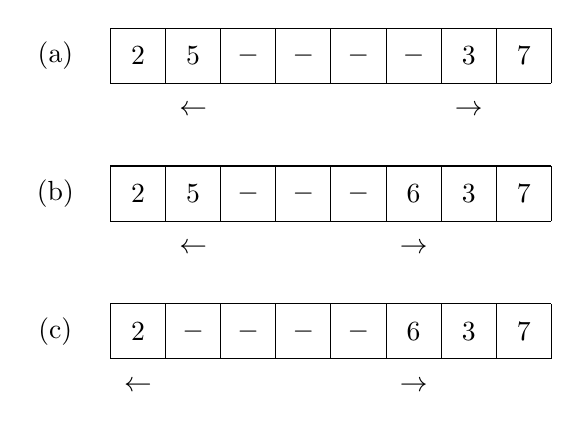
\begin{tikzpicture}[scale=0.7]
\begin{scope}
\draw (0,0) grid (8,1);
\node at (-1,0.5) {(a)};
\node at (0.5,0.5) {$2$};
\node at (1.5,0.5) {$5$};
\node at (2.5,0.5) {$-$};
\node at (3.5,0.5) {$-$};
\node at (4.5,0.5) {$-$};
\node at (5.5,0.5) {$-$};
\node at (6.5,0.5) {$3$};
\node at (7.5,0.5) {$7$};
\node at (1.5,-0.5) {$\leftarrow$};
\node at (6.5,-0.5) {$\rightarrow$};
\end{scope}
\begin{scope}[yshift=-2.5cm]
\draw (0,0) grid (8,1);
\node at (-1,0.5) {(b)};
\node at (0.5,0.5) {$2$};
\node at (1.5,0.5) {$5$};
\node at (2.5,0.5) {$-$};
\node at (3.5,0.5) {$-$};
\node at (4.5,0.5) {$-$};
\node at (5.5,0.5) {$6$};
\node at (6.5,0.5) {$3$};
\node at (7.5,0.5) {$7$};
\node at (1.5,-0.5) {$\leftarrow$};
\node at (5.5,-0.5) {$\rightarrow$};
\end{scope}
\begin{scope}[yshift=-5cm]
\draw (0,0) grid (8,1);
\node at (-1,0.5) {(c)};
\node at (0.5,0.5) {$2$};
\node at (1.5,0.5) {$-$};
\node at (2.5,0.5) {$-$};
\node at (3.5,0.5) {$-$};
\node at (4.5,0.5) {$-$};
\node at (5.5,0.5) {$6$};
\node at (6.5,0.5) {$3$};
\node at (7.5,0.5) {$7$};
\node at (0.5,-0.5) {$\leftarrow$};
\node at (5.5,-0.5) {$\rightarrow$};
\end{scope}
\end{tikzpicture}
\caption{(a) Lista $[3,7,2,5]$ tallennettuna taulukkoon.
(b) Listan alkuun lisätään alkio 6.
(c) Listan lopusta poistetaan alkio 5.}
\label{fig:lismol}
\end{figure}

Kuva \ref{fig:lismol} näyttää esimerkin listan $[3,7,2,5]$
uudesta tallennustavasta.
Merkki $\rightarrow$ osoittaa kohdan, josta lista alkaa,
ja merkki $\leftarrow$ osoittaa kohdan, johon lista päättyy.
Kun haluamme lisätä alkion listan alkuun,
siirrymme vasemmalle kohdasta $\rightarrow$,
ja kun haluamme lisätä alkion listan loppuun,
siirrymme oikealle kohdasta $\leftarrow$.
Kun haluamme poistaa alkioita listasta,
menettelemme käänteisesti.

Jos kohdat $\leftarrow$ ja $\rightarrow$ ovat vierekkäin
tässä järjestyksessä, tämä voi tarkoittaa kahta asiaa:
joko lista on tyhjä tai sitten kaikki taulukon kohdat ovat käytössä.
Kuva \ref{fig:lismol2} näyttää esimerkin näistä tilanteista.
Kun pidämme muistissa alkioiden määrää,
voimme päätellä siitä, kumpi tilanne on kyseessä.
Jos taulukko on täynnä ja haluamme lisätä uuden alkion,
meidän täytyy varata uusi suurempi taulukko, johon listan sisältö siirretään.
Voimme menetellä samalla tavalla kuin aiemmin ja
esimerkiksi kaksinkertaistaa taulukon koon joka vaiheessa,
jolloin operaatiot vievät keskimäärin aikaa $O(1)$.

\begin{figure}
\center
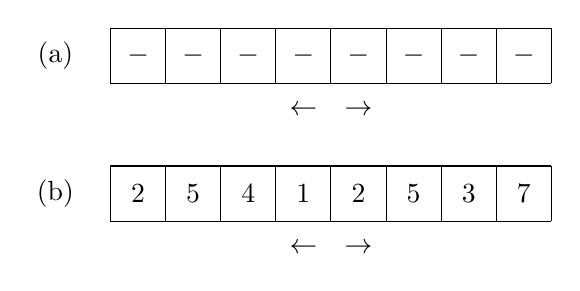
\begin{tikzpicture}[scale=0.7]
\begin{scope}
\draw (0,0) grid (8,1);
\node at (-1,0.5) {(a)};
\node at (0.5,0.5) {$-$};
\node at (1.5,0.5) {$-$};
\node at (2.5,0.5) {$-$};
\node at (3.5,0.5) {$-$};
\node at (4.5,0.5) {$-$};
\node at (5.5,0.5) {$-$};
\node at (6.5,0.5) {$-$};
\node at (7.5,0.5) {$-$};
\node at (3.5,-0.5) {$\leftarrow$};
\node at (4.5,-0.5) {$\rightarrow$};
\end{scope}
\begin{scope}[yshift=-2.5cm]
\draw (0,0) grid (8,1);
\node at (-1,0.5) {(b)};
\node at (0.5,0.5) {$2$};
\node at (1.5,0.5) {$5$};
\node at (2.5,0.5) {$4$};
\node at (3.5,0.5) {$1$};
\node at (4.5,0.5) {$2$};
\node at (5.5,0.5) {$5$};
\node at (6.5,0.5) {$3$};
\node at (7.5,0.5) {$7$};
\node at (3.5,-0.5) {$\leftarrow$};
\node at (4.5,-0.5) {$\rightarrow$};
\end{scope}
\end{tikzpicture}
\caption{Kaksi samantapaista tilannetta:
(a) Listassa ei ole yhtään alkiota.
(b) Listan alkiot täyttävät koko taulukon.}
\label{fig:lismol2}
\end{figure}

\section{Linkitetty lista}

\index{linkitetty lista}

\emph{Linkitetty lista} (\emph{linked list}) muodostuu solmuista, joista jokainen sisältää
yhden listan alkion.
Linkitetty lista voi olla yhteen tai kahteen suuntaan linkitetty.
Yhteen suuntaan linkitetyssä listassa jokaisesta solmusta
on viittaus seuraavaan solmuun, ja kahteen suuntaan linkitetyssä
listassa jokaisesta solmusta on viittaus sekä seuraavaan että edelliseen solmuun.

\begin{figure}
\center
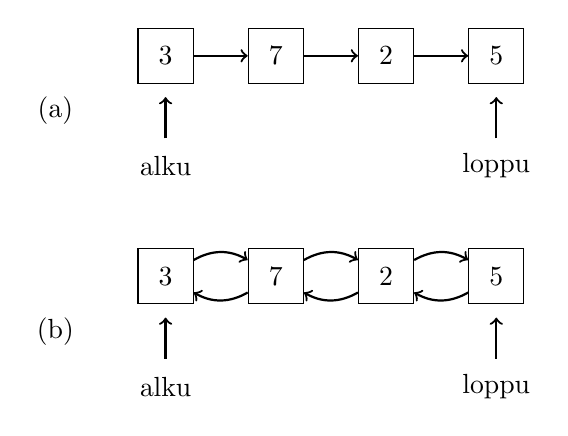
\begin{tikzpicture}[scale=0.7]
\begin{scope}
\node[draw, rectangle, minimum size=7mm] (1) at (0,0) {$3$};
\node[draw, rectangle, minimum size=7mm] (2) at (2,0) {$7$};
\node[draw, rectangle, minimum size=7mm] (3) at (4,0) {$2$};
\node[draw, rectangle, minimum size=7mm] (4) at (6,0) {$5$};
\path[draw,thick,->] (1) -- (2);
\path[draw,thick,->] (2) -- (3);
\path[draw,thick,->] (3) -- (4);
\node at (0,-2) {alku};
\node at (6,-2) {loppu};
\path[draw,thick,->] (0,-1.5) -- (0,-0.75);
\path[draw,thick,->] (6,-1.5) -- (6,-0.75);
\node at (-2,-1) {(a)};
\end{scope}
\begin{scope}[yshift=-4cm]
\node[draw, rectangle, minimum size=7mm] (1) at (0,0) {$3$};
\node[draw, rectangle, minimum size=7mm] (2) at (2,0) {$7$};
\node[draw, rectangle, minimum size=7mm] (3) at (4,0) {$2$};
\node[draw, rectangle, minimum size=7mm] (4) at (6,0) {$5$};
\path[draw,thick,->] (1) edge [bend left] (2);
\path[draw,thick,->] (2) edge [bend left] (3);
\path[draw,thick,->] (3) edge [bend left] (4);
\path[draw,thick,->] (4) edge [bend left] (3);
\path[draw,thick,->] (3) edge [bend left] (2);
\path[draw,thick,->] (2) edge [bend left] (1);
\node at (0,-2) {alku};
\node at (6,-2) {loppu};
\path[draw,thick,->] (0,-1.5) -- (0,-0.75);
\path[draw,thick,->] (6,-1.5) -- (6,-0.75);
\node at (-2,-1) {(b)};
\end{scope}
\end{tikzpicture}
\caption{Lista $[3,7,2,5]$ linkitettynä listana.
(a) Yhteen suuntaan linkitetty lista. (b) Kahteen suuntaan linkitetty lista.}
\label{fig:linlis}
\end{figure}

Kuva \ref{fig:linlis} näyttää esimerkkinä listan $[3,7,2,5]$
yhteen ja kahteen suuntaan linkitettynä.
Molemmissa listoissa tiedossa on viittaukset listan
alkuun ja loppuun.
Yhteen suuntaan linkitetyssä listassa voimme käydä
läpi listan alkiot alusta loppuun,
kun taas kahteen suuntaan linkitetyssä listassa
voimme kulkea sekä alusta loppuun että lopusta alkuun.

Tavallinen tapa toteuttaa linkitetty rakenne ohjelmointikielissä
on luoda luokka, jonka oliot vastaavat rakenteen solmuja.
Esimerkiksi voisimme rakentaa yhteen suuntaan
linkitetyn listan $[1,2,3]$ tähän tapaan:

\begin{code}
a.arvo = 1
a.seuraava = b
b.arvo = 2
b.seuraava = c
c.arvo = 3
c.seuraava = null
\end{code}

Tässä toteutuksessa jokaisessa solmuoliossa on kaksi kenttää:
\texttt{arvo} on solmussa oleva arvo ja
\texttt{seuraava} viittaa listan seuraavaan solmuun.
Listan loppumisen ilmaisee viimeisessä solmussa oleva arvo \texttt{null}.
Voisimme käydä läpi listan solmut näin:

\begin{code}
s = a
while s != null
    print(s.arvo)
    s = s.seuraava
\end{code}

\subsection{Listan operaatiot}

Käytännössä järkevä tapa toteuttaa linkitetty lista on tehdä
listasta kaksisuuntainen, jolloin tiedämme jokaisessa solmussa
seuraavan ja edellisen solmun ja voimme kulkea listaa molempiin suuntiin.

Linkitetyn listan etuna on,
että voimme lisätä ja poistaa
alkioita $O(1)$-ajassa kaikissa listan kohdissa.
Kun haluamme lisätä listalle alkion,
luomme ensin uuden solmun ja muutamme sitten
sen vieressä olevien solmujen viittauksia niin,
että ne viittaavat uuteen solmuun.
Vastaavasti kun haluamme poistaa alkion,
muutamme viittauksia niin, että solmu ohitetaan.

\begin{figure}
\center
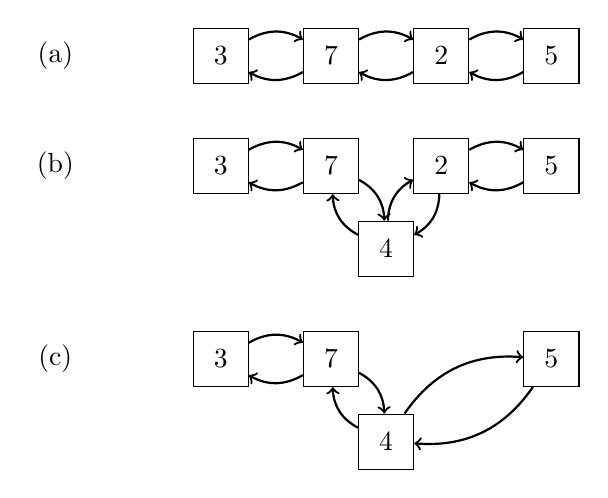
\begin{tikzpicture}[scale=0.7]
\begin{scope}
\node at (-3,0) {(a)};
\node[draw, rectangle, minimum size=7mm] (1) at (0,0) {$3$};
\node[draw, rectangle, minimum size=7mm] (2) at (2,0) {$7$};
\node[draw, rectangle, minimum size=7mm] (3) at (4,0) {$2$};
\node[draw, rectangle, minimum size=7mm] (4) at (6,0) {$5$};
\path[draw,thick,->] (1) edge [bend left] (2);
\path[draw,thick,->] (2) edge [bend left] (3);
\path[draw,thick,->] (3) edge [bend left] (4);
\path[draw,thick,->] (4) edge [bend left] (3);
\path[draw,thick,->] (3) edge [bend left] (2);
\path[draw,thick,->] (2) edge [bend left] (1);
\end{scope}
\begin{scope}[yshift=-2cm]
\node at (-3,0) {(b)};
\node[draw, rectangle, minimum size=7mm] (1) at (0,0) {$3$};
\node[draw, rectangle, minimum size=7mm] (2) at (2,0) {$7$};
\node[draw, rectangle, minimum size=7mm] (3) at (4,0) {$2$};
\node[draw, rectangle, minimum size=7mm] (4) at (6,0) {$5$};
\node[draw, rectangle, minimum size=7mm] (5) at (3,-1.5) {$4$};
\path[draw,thick,->] (1) edge [bend left] (2);
\path[draw,thick,->] (2) edge [bend left] (5);
\path[draw,thick,->] (5) edge [bend left] (3);
\path[draw,thick,->] (3) edge [bend left] (4);
\path[draw,thick,->] (4) edge [bend left] (3);
\path[draw,thick,->] (3) edge [bend left] (5);
\path[draw,thick,->] (5) edge [bend left] (2);
\path[draw,thick,->] (2) edge [bend left] (1);
\end{scope}
\begin{scope}[yshift=-5.5cm]
\node at (-3,0) {(c)};
\node[draw, rectangle, minimum size=7mm] (1) at (0,0) {$3$};
\node[draw, rectangle, minimum size=7mm] (2) at (2,0) {$7$};
\node[draw, rectangle, minimum size=7mm] (4) at (6,0) {$5$};
\node[draw, rectangle, minimum size=7mm] (5) at (3,-1.5) {$4$};
\path[draw,thick,->] (1) edge [bend left] (2);
\path[draw,thick,->] (2) edge [bend left] (5);
\path[draw,thick,->] (5) edge [bend left] (4);
\path[draw,thick,->] (4) edge [bend left] (5);
\path[draw,thick,->] (5) edge [bend left] (2);
\path[draw,thick,->] (2) edge [bend left] (1);
\end{scope}
\end{tikzpicture}
\caption{(a) Alkuperäinen lista $[3,7,2,5]$.
(b) Listan keskelle lisätään alkio $4$.
(c) Listasta poistetaan alkio $2$.}
\label{fig:lismuu}
\end{figure}

Kuva \ref{fig:lismuu} näyttää esimerkin linkitetyn listan käsittelystä.
Listan sisältönä on aluksi $[3,7,2,5]$.
Sitten lisämme listan keskelle alkion 4,
jolloin luomme ensin uuden solmun alkiolle ja muutamme
sitten viittauksia alkioiden 7 ja 2 välillä niin,
että alkio 4 tulee niiden väliin.
Lopuksi poistamme listasta alkion 2, jolloin yhdistämme
alkiot 4 ja 5 suoraan toisiinsa.

Pääsemme listan ensimmäiseen ja viimeiseen solmuun tehokkaasti,
koska muistissa on viittaukset niihin.
Sen sijaan jos haluamme päästä johonkin muuhun listan kohtaan,
matka täytyy aloittaa listan alusta tai lopusta ja kulkea askel
kerrallaan viittauksia seuraten.
Niinpä listan keskellä olevaan kohtaan pääseminen vie aikaa $O(n)$.
Joudumme liikkumaan solmuihin linkkejä pitkin, koska solmut voivat
olla eri puolilla muistia eikä ole keinoa tietää suoraan,
mihin mikäkin solmu on tallennettu.

\subsection{Listojen vertailua}

\begin{table}
\center
\begin{tabular}{lrr}
operaatio & taulukkolista & linkitetty lista \\
\hline
pääsy listan alkuun & $O(1)$ & $O(1)$ \\
pääsy listan loppuun & $O(1)$ & $O(1)$ \\ 
pääsy listan keskelle &  $O(1)$ & $O(n)$ \\
lisäys/poisto listan alussa & $O(1)$ & $O(1)$ \\
lisäys/poisto listan lopussa & $O(1)$ & $O(1)$ \\ 
lisäys/poisto listan keskellä &  $O(n)$ & $O(1)$ \\
\end{tabular}
\caption{Taulukkolistan ja linkitetyn listan aikavaativuuksia.}
\label{tab:taulin}
\end{table}

Taulukko \ref{tab:taulin} esittää yhteenvedon taulukkolistan ja
linkitetyn listan ominaisuuksista.
Kummassakin toteutuksessa on yksi operaatio,
joka ei ole tehokas.
Taulukkolistassa pääsemme tehokkaasti mihin tahansa listan
kohtaan, mutta on hidasta muokata listaa keskeltä.
Linkitetyssä listassa voimme helposti muokata listaa mistä tahansa,
mutta keskelle pääseminen on hidasta.

Huomaa, että keskelle pääsemisen hitaus rajoittaa melko paljon
linkitetyn listan käyttämistä.
Vaikka pystymme sinänsä muokkaamaan listaa mistä tahansa kohdasta
tehokkaasti, meidän tulee ensin \emph{päästä} kyseiseen kohtaan.
Jos jostain syystä on etukäteen tiedossa viittaus listan keskelle,
voimme muokata kyseistä kohtaa tehokkaasti,
mutta muuten tulee ensin kulkea haluttuun kohtaan,
missä kuluu aikaa $O(n)$.

\section{Pino ja jono}

Listan avulla voimme toteuttaa myös kaksi erikoistunutta tietorakennetta,
pinon ja jonon, jotka sisältävät vain osan listan ominaisuuksista
eli niiden operaatiot ovat listaa rajoittuneempia.

\begin{figure}
\center
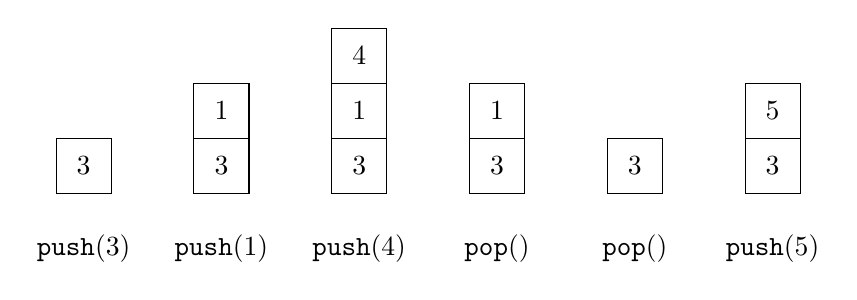
\begin{tikzpicture}[scale=0.7]
\begin{scope}[xshift=2.5cm]
\draw (0,0) grid (1,1);
\node at (0.5,0.5) {3};
\node at (0.5,-1) {$\texttt{push}(3)$};
\end{scope}
\begin{scope}[xshift=5cm]
\draw (0,0) grid (1,2);
\node at (0.5,0.5) {3};
\node at (0.5,1.5) {1};
\node at (0.5,-1) {$\texttt{push}(1)$};
\end{scope}
\begin{scope}[xshift=7.5cm]
\draw (0,0) grid (1,3);
\node at (0.5,0.5) {3};
\node at (0.5,1.5) {1};
\node at (0.5,2.5) {4};
\node at (0.5,-1) {$\texttt{push}(4)$};
\end{scope}
\begin{scope}[xshift=10cm]
\draw (0,0) grid (1,2);
\node at (0.5,0.5) {3};
\node at (0.5,1.5) {1};
\node at (0.5,-1) {$\texttt{pop}()$};
\end{scope}
\begin{scope}[xshift=12.5cm]
\draw (0,0) grid (1,1);
\node at (0.5,0.5) {3};
\node at (0.5,-1) {$\texttt{pop}()$};
\end{scope}
\begin{scope}[xshift=15cm]
\draw (0,0) grid (1,2);
\node at (0.5,0.5) {3};
\node at (0.5,1.5) {5};
\node at (0.5,-1) {$\texttt{push}(5)$};
\end{scope}
\end{tikzpicture}
\caption{Esimerkki pinon käsittelystä:
lisäämme tyhjään pinoon alkiot 3, 1 ja 4, poistamme kaksi ylintä
alkiota ja lisäämme lopuksi alkion 5.}
\label{fig:pinesi}
\end{figure}

\begin{figure}
\center
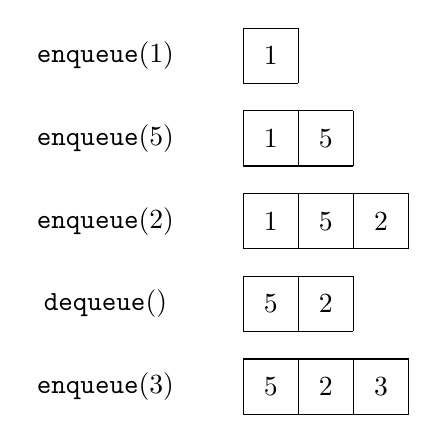
\begin{tikzpicture}[scale=0.7]
\begin{scope}
\draw (0,0) grid (1,1);
\node at (0.5,0.5) {$1$};
\node at (-2.5,0.5) {$\texttt{enqueue}(1)$};
\end{scope}
\begin{scope}[yshift=-1.5cm]
\draw (0,0) grid (2,1);
\node at (0.5,0.5) {$1$};
\node at (1.5,0.5) {$5$};
\node at (-2.5,0.5) {$\texttt{enqueue}(5)$};
\end{scope}
\begin{scope}[yshift=-3cm]
\draw (0,0) grid (3,1);
\node at (0.5,0.5) {$1$};
\node at (1.5,0.5) {$5$};
\node at (2.5,0.5) {$2$};
\node at (-2.5,0.5) {$\texttt{enqueue}(2)$};
\end{scope}
\begin{scope}[yshift=-4.5cm]
\draw (0,0) grid (2,1);
\node at (0.5,0.5) {$5$};
\node at (1.5,0.5) {$2$};
\node at (-2.5,0.5) {$\texttt{dequeue}()$};
\end{scope}
\begin{scope}[yshift=-6cm]
\draw (0,0) grid (3,1);
\node at (0.5,0.5) {$5$};
\node at (1.5,0.5) {$2$};
\node at (2.5,0.5) {$3$};
\node at (-2.5,0.5) {$\texttt{enqueue}(3)$};
\end{scope}
\end{tikzpicture}
\caption{Esimerkki jonon käsittelystä:
lisäämme tyhjään jonon alkiot 1, 5 ja 2,
poistamme yhden alkion ja lisäämme vielä alkion 3.}
\label{fig:jonesi}
\end{figure}

\index{pino}

\emph{Pino} (\emph{stack}) on tietorakenne,
jonka operaatiot ovat
alkion lisääminen pinon päälle (\texttt{push}),
ylimmän alkion poistaminen (\texttt{pop})
sekä ylimmän alkion hakeminen.
Esimerkiksi kuvassa \ref{fig:pinesi} lisäämme ensin tyhjään pinoon kolme alkiota,
poistamme sitten kaksi alkiota ja lisäämme vielä yhden alkion.

\index{jono}

\emph{Jono} (\emph{queue}) on tietorakenne, jossa voimme lisätä alkioita
jonon loppuun (\texttt{enqueue}),
poistaa alkioita jonon alusta (\texttt{dequeue})
ja hakea alkioita molemmista päistä.
Esimerkiksi kuvassa \ref{fig:jonesi} lisäämme ensin tyhjään jonoon
kolme alkiota, poistamme sitten yhden alkion ja lisämme vielä yhden alkion.

Pystymme toteuttamaan sekä pinon että jonon helposti
listana niin, että niiden operaatiot toimivat ajassa $O(1)$.
Mutta mitä järkeä on luoda uusia tietorakenteita,
jotka ovat \emph{huonompia} kuin lista?
Listassa voimme käsitellä mitä tahansa alkioita, mutta
pinossa ja jonossa emme pääse käsiksi keskellä oleviin alkioihin.
Selitys on siinä, että pino ja jono ovat hyödyllisiä 
\emph{käsit\-teitä} algoritmien suunnittelussa.
Voimme usein ajatella algoritmissa tarvittavaa
tietorakennetta pinona tai jonona ja toteuttaa sen sitten listana.

Tarkastellaan esimerkkinä ongelmaa, jossa annettuna on
$n$ merkin pituinen \emph{sulkulauseke}, 
joka muodostuu kaarisulkeista \texttt{(} ja \texttt{)} sekä
hakasulkeista \texttt{[} ja \texttt{]}.
Haluamme selvittää, onko lauseke \emph{oikein muodostettu} eli
onko jokaiselle aloittavalle sululle vastaava lopettava pari.
Esimerkiksi lauseke \texttt{[()]()} on oikein muodostettu,
kun taas lauseke \texttt{[()(])} ei ole.
Voimme ratkaista ongelman $O(n)$-ajassa pinon avulla
käymällä läpi lausekkeen merkit vasemmalta oikealle.
Kun vastaan tulee aloittava sulku \texttt{(} tai \texttt{[},
lisäämme sen pinoon.
Kun taas vastaan tulee lopettava sulku \texttt{)} tai \texttt{]},
tutkimme, mikä on pinossa ylimpänä oleva merkki.
Jos merkki on vastaava aloittava sulku,
poistamme sen pinosta, ja muuten toteamme, että lauseke on virheellinen.
Jos lausekkeen läpikäynnin aikana ei esiinny virheitä
ja pino on lopuksi tyhjä, lauseke on oikein muodostettu.

\section{Ohjelmointikielten toteutukset}

\subsection{Java}

Javan \texttt{ArrayList} on taulukkolista,
jossa alkion lisääminen ja poistaminen on tehokasta,
kun se tapahtuu listan lopussa.
Metodi \texttt{add} lisää tehokkaasti alkion listan loppuun:

\begin{code}
ArrayList<Integer> lista = new ArrayList<>();
lista.add(1);
lista.add(2);
lista.add(3);
// tulos: [1,2,3]
\end{code}

Metodi \texttt{remove} poistaa alkion
annetusta listan kohdasta.
Metodi toimii tehokkaasti, kun poistokohta on listan lopussa.
Esimerkiksi seuraava koodi poistaa listan viimeisen alkion:

\begin{code}
lista.remove(lista.size()-1);
\end{code}

Koska lista on tallennettu taulukkona,
pääsemme myös tehokkaasti käsiksi missä tahansa kohdassa
olevaan alkioon metodeilla \texttt{get} ja \texttt{set}:

\begin{code}
// hae alkio kohdasta 3
int x = lista.get(3);
// muuta kohdan 5 alkioksi 8
lista.set(5,8);
\end{code}

\texttt{ArrayDeque} on taulukkolista,
joka sallii tehokkaat lisäykset ja poistot
sekä listan alussa että lopussa.
Metodit \texttt{addFirst} ja \texttt{addLast}
lisäävät alkioita,
ja metodit \texttt{removeFirst} ja \texttt{removeLast}
poistavat alkioita.

\begin{code}
ArrayDeque<Integer> lista = new ArrayDeque<>();
lista.addLast(1);
lista.addLast(2);
lista.addLast(3);
lista.removeFirst();
lista.addFirst(4);
// tulos: [4,2,3]
\end{code}

Lisäksi voimme hakea listan ensimmäisen ja viimeisen alkion
metodeilla \texttt{getFirst} ja \texttt{getLast}:

\begin{code}
int eka = lista.getFirst();
int vika = lista.getLast();
\end{code}

Rajoituksena on kuitenkin, että yleisiä metodeita
\texttt{get} ja \texttt{set} ei ole tarjolla
eli emme pääse tehokkaasti käsiksi listan keskellä
oleviin alkioihin.

\texttt{LinkedList} on kaksisuuntainen linkitetty lista,
jota voimme käsitellä samaan tapaan kuin \texttt{ArrayDeque}-listaa:

\begin{code}
LinkedList<Integer> lista = new LinkedList<>();
lista.addLast(1);
lista.addLast(2);
lista.addLast(3);
lista.removeFirst();
lista.addFirst(4);
// tulos: [4,2,3]
\end{code}

\texttt{LinkedList} tarjoaa myös metodit
\texttt{get} ja \texttt{set}, joiden avulla
pääsee käsiksi tietyssä kohdassa listalla olevaan alkioon.
Nämä metodit vievät kuitenkin aikaa $O(n)$,
koska joudumme kulkemaan ensin oikeaan kohtaan listan
alusta tai lopusta.

\index{iteraattori}

Voimme käsitellä listaa myös \emph{iteraattorilla}
(\emph{iterator}),
joka osoittaa tiettyyn listan kohtaan.
Esimerkiksi seuraava koodi luo iteraattorin,
joka osoittaa listan alkuun,
siirtää iteraattoria kaksi askelta eteenpäin ja
lisää alkion iteraattorin kohdalle eli listan
toisen ja kolmannen alkion väliin.

\begin{code}
ListIterator<Integer> x = lista.listIterator();
x.next();
x.next();
x.add(5);
\end{code}

Iteraattorin avulla voimme muokata tehokkaasti
linkitettyä listaa siitä kohdasta,
jossa iteraattori on tällä hetkellä.

\subsection{Python}

Pythonin tavallinen lista on taulukkolista,
jota voi käsitellä tehokkaasti listan lopusta.
Metodi \texttt{append} lisää alkion listan loppuun:

\begin{code}
lista = []
lista.append(1)
lista.append(2)
lista.append(3)
# tulos: [1,2,3]
\end{code}

Metodi \texttt{pop} puolestaan poistaa listan viimeisen alkion:

\begin{code}
lista.pop()
\end{code}

Pääsemme käsiksi listan alkioihin tehokkaasti \texttt{[]}-syntaksin avulla:

\begin{code}
x = lista[3]
lista[5] = 8
\end{code}

Pythonissa on myös lista \texttt{deque},
joka on toteutettu linkitettynä listana.
Lisäykset ja poistot ovat tehokkaita sekä listan
alussa että lopussa.
Saamme tietorakenteen käyttöön näin:

\begin{code}
from collections import deque
\end{code}

Tavallisen listan tavoin \texttt{deque} tarjoaa
metodit \texttt{append} ja \texttt{pop},
mutta lisäksi siinä on metodit \texttt{appendleft}
ja \texttt{popleft}, joiden avulla voi lisätä ja poistaa
alkioita listan alussa:

\begin{code}
lista = deque()
lista.append(1)
lista.append(2)
lista.append(3)
lista.popleft()
lista.appendleft(4)
# tulos: [4,2,3]
\end{code}

Listan alkuun ja loppuun pääsee käsiksi näin:

\begin{code}
eka = lista[0]
vika = lista[-1]
\end{code}

Myös listan keskellä olevia alkioita voi käsitellä \texttt{[]}-syntaksilla,
mutta tämä vie aikaa $O(n)$, koska kyseessä on linkitetty lista.

\section{Miten valita lista?}

Voimme käyttää usein algoritmin toteutukseen joko
taulukkolistaa tai linkitettyä listaa ja saada aikaan
aikavaativuuden kannalta yhtä tehokkaan algoritmin.
Esimerkiksi jos algoritmi lisää listan loppuun alkioita,
sekä taulukkolistassa että linkitetyssä listassa
lisäämisen aikavaativuus on $O(1)$.
Mutta kumpi lista on parempi valinta käytännössä?

\begin{figure}
\center
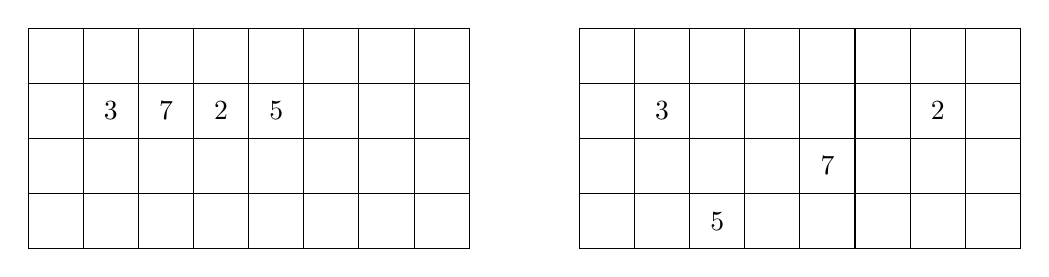
\begin{tikzpicture}[scale=0.7]
\begin{scope}
\draw (0,0) grid (8,4);
\node at (1.5,2.5) {3};
\node at (2.5,2.5) {7};
\node at (3.5,2.5) {2};
\node at (4.5,2.5) {5};
\end{scope}
\begin{scope}[xshift=10cm]
\draw (0,0) grid (8,4);
\node at (1.5,2.5) {3};
\node at (4.5,1.5) {7};
\node at (6.5,2.5) {2};
\node at (2.5,0.5) {5};
\end{scope}
\end{tikzpicture}
\caption{Taulukkolista ja linkitetty lista tietokoneen muistissa.}
\label{fig:taulin}
\end{figure}

Useimmissa tapauksissa parempi valinta on taulukkolista,
koska nykyaikaiset tietokoneet
\emph{suosivat} taulukkolistan käyttämistä linkitetyn listan sijaan.
Kuvassa \ref{fig:taulin} näkyy, miten taulukkolista ja linkitetty lista
asettuvat tietokoneen muistissa.
Taulukkolistan alkiot ovat peräkkäin, kun taas linkitetyn
listan alkiot voivat olla eri puolilla muistia sekalaisessa
järjestyksessä.
Nykyaikaisen prosessorin välimuistit ja seuraavaksi suoritettavien
komentojen ennustus
on toteutettu niin, että ne ovat parhaimmillaan silloin,
kun tieto on tallennettu muistissa peräkkäin -- eli juuri kuten
taulukkolistassa.
Tämä näkyy käytännössä siinä, että taulukkolistan käsittely on selvästi
tehokkaampaa kuin linkitetyn listan käsittely.

Vaikka linkitetty lista ei ole usein käytännössä hyvä tietorakenne,
linkitetyn rakenteen idea on hyödyllinen
ja tarvitsemme sitä myöhemmin monimutkaisemmissa tietorakenteissa.
